% Doc class
\documentclass[11pt, a4paper, onecolumn, logo, copyright]{googledeepmind}
\pdfoutput=1


% Omit dates for reproducibility.
%\pdfinfoomitdate 1
%\pdftrailerid{redacted}

% هذا يتجنب إدخالات المرجعية المكررة عند استخدام \bibentry (على سبيل المثال عبر \citeas).
\makeatletter
\renewcommand\bibentry[1]{\nocite{#1}{\frenchspacing@nameuse{BR@r@#1@extra@b@citeb}}}
\makeatother

\usepackage[authoryear, sort&compress, round]{natbib}
\bibliographystyle{abbrvnat}

\usepackage{amsmath}
% \usepackage{minted}

% معلومات حول مستندك.
\title{مزيج الأعماق: تخصيص الحوسبة ديناميكيًا في نماذج اللغة القائمة على المحولات}

% يمكن ترك هذا الخيار إذا لم ترغب في إضافة مؤلف مراسل.
\correspondingauthor{draposo@google.com, adamsantoro@google.com}

% قم بتعيين تاريخك الخاص للتقرير.
% يمكن التعليق إذا لم تكن هناك حاجة أو ترك فارغًا إذا كان لا ينطبق.
\renewcommand{\today}{}

% يمكن أن يكون هناك عدد من المؤلفين والانتماءات حسب الحاجة. الأفضل الإشارة إلى
% التأليف المشترك الأول كما هو موضح أدناه.
\author[1*]{ديفيد رابوسو}
\author[1]{سام ريتر}
\author[1,2]{بليك ريتشاردز}
\author[1]{تيموثي ليليكراب}
\author[1]{بيتر كونواي هامفريز}
\author[1*]{آدم سانتورو}

% يجب أن تأتي الانتماءات بعد إعلان \author[]
\affil[1]{جوجل ديب مايند}
\affil[2]{جامعة ماكجيل ومعهد ميلا}
\affil[*]{مساهمة متساوية}

\begin{abstract}
تنشر نماذج لغة المحولات عمليات FLOP بشكل موحد عبر تسلسلات الإدخال. في هذا العمل، نوضح أن المحولات يمكنها بدلاً من ذلك أن تتعلم تخصيص FLOPs (أو \emph{الحوسبة}) ديناميكيًا لمواضع محددة في التسلسل، وتحسين التخصيص على طول التسلسل لطبقات مختلفة عبر عمق النموذج. تفرض طريقتنا ميزانية حوسبة إجمالية عن طريق تحديد عدد الرموز المميزة ($k$) التي يمكن أن تشارك في حسابات الاهتمام الذاتي و MLP عند طبقة معينة. يتم تحديد الرموز المميزة التي سيتم معالجتها بواسطة الشبكة باستخدام آلية توجيه أعلى $k$. بما أن $k$ محدد \emph{مسبقًا}، تستخدم هذه الإجراء البسيط رسم بياني حسابي ثابت مع أحجام مِصفوفية معروفة، على عكس تقنيات الحوسبة الشرطية الأخرى. ومع ذلك، نظرًا لأن هويات الرموز المميزة $k$ سائلة، يمكن لهذه الطريقة أن تنفق FLOPs بشكل غير موحد عبر أبعاد الوقت وعمق النموذج. وبالتالي، فإن إنفاق الحوسبة يمكن التنبؤ به تمامًا في المجموع، ولكنه ديناميكي وحساس للسياق على مستوى الرمز المميز. ليس فقط النماذج المدربة بهذه الطريقة تتعلم تخصيص الحوسبة ديناميكيًا، ولكنها تفعل ذلك بكفاءة. تطابق هذه النماذج أداء الأساس لـ FLOPS المكافئة وأوقات الساعة الحائطية للتدريب، ولكنها تتطلب جزءًا من FLOPs لكل تمرير أمامي، ويمكن أن تكون أسرع بنسبة 50٪ في الخطوة أثناء أخذ العينات بعد التدريب.
\end{abstract}

\begin{document}

\maketitle

\section{مقدمة}
لا تتطلب جميع المشكلات نفس الوقت أو الجهد للحل. وبالمثل، في نمذجة اللغة، لا تتطلب جميع الرموز المميزة والتسلسلات نفس الوقت أو الجهد للتنبؤ الدقيق. ومع ذلك، تنفق نماذج المحولات نفس كمية الحوسبة لكل رمز مميز في التمرير الأمامي. من الناحية المثالية، يجب أن تستخدم المحولات ميزانيات حوسبة إجمالية أصغر من خلال عدم إنفاق الحوسبة بلا داعٍ.

تعد الحوسبة الشرطية تقنية تحاول تقليل إجمالي الحوسبة من خلال إنفاقها فقط عند الحاجة \citep{bengio2013deep,bengio2013estimating,bengio2016conditional}. تقدم الخوارزميات المختلفة حلولاً لمتى وكم ينبغي استخدام الحوسبة \citep{ainslie2023colt5, fedus2022switch, bapna_controlling}. ومع ذلك، قد لا تعمل الصيغ العامة لهذه المشكلة الصعبة بشكل جيد مع قيود الأجهزة الحالية نظرًا لأنها تميل إلى إدخال رسوم بيانية حسابية ديناميكية \citep{graves_adaptive, dehghani2018universal}. قد تكون أساليب الحوسبة الشرطية الأكثر واعدة هي تلك المتناغمة مع مكدس أجهزتنا الحالية، والتي تعطي الأولوية للرسوم البيانية الحسابية الثابتة، وأحجام المِصفوفات المعروفة التي يتم اختيارها لتعظيم استخدام الأجهزة.

هنا نأخذ بعين الاعتبار مشكلة نمذجة اللغة باستخدام ميزانية \textit{ثابتة} يمكن جعلها أقل من تلك المستخدمة من قبل محول عادي. يجب على الشبكة أن تتعلم كيفية \textit{تخصيص} الحوسبة المتاحة ديناميكيًا من خلال اتخاذ قرارات لكل رمز مميز، في كل طبقة، حول مكان إنفاق الحوسبة من الميزانية المتاحة. في تنفيذنا، يتم تحديد إجمالي الحوسبة من قبل المستخدم ولا تتغير قبل التدريب، بدلاً من أن تكون دالة في قرارات الشبكة أثناء العمل. وبالتالي، يمكن توقع المكاسب في كفاءة الأجهزة - مثل تقليل البصمة الذاكرية، أو تقليل FLOPs لكل تمرير أمامي - واستغلالها مسبقًا. كما سنوضح، يمكن الحصول على هذه المكاسب دون التضحية بالأداء العام.

نستفيد من نهج يشبه محولات خليط من الخبراء (MoE)، حيث يتم اتخاذ قرارات توجيه ديناميكية على مستوى الرمز المميز عبر عمق الشبكة. خلافًا لـ MoE، نختار إما تطبيق حساب على الرمز المميز (كما هو الحال بالنسبة للمحول القياسي)، أو تمريره عبر اتصال متبقٍ (يظل دون تغيير وتوفير الحوسبة). أيضًا على عكس MoE، نطبق هذا التوجيه على كل من MLPs الأمامية والانتباه متعدد الرؤوس. نظرًا لأن هذا يؤثر أيضًا على المفاتيح والاستعلامات التي نعالجها، يتخذ التوجيه قرارات ليس فقط حول الرموز المميزة التي يتم تحديثها، ولكن أيضًا الرموز المميزة التي يتم إتاحتها للانتباه إليها. نشير إلى هذه الإستراتيجية باسم مزيج الأعماق (MoD) للتأكيد على كيفية مرور الرموز المميزة الفردية عبر عدد مختلف من الطبقات، أو الكتل، خلال عمق المحول (انظر الشكل \ref{fig:mixture-of-depths}).

تسمح تقنية MoD أيضًا بالمفاضلة بين الأداء والسرعة. من ناحية، يمكن للمرء تدريب محول MoD يحسن من المحولات العادية بنسبة تصل إلى 1.5٪ على هدف التدريب النهائي لاحتمالات السجل لـ FLOPs المكافئة (isoFLOP)، وبينما يستغرق نفس الوقت على الساعة الحائطية للتدريب. من ناحية أخرى، يمكن للمرء تدريب محول MoD يحقق تكافؤ خسارة التدريب مع محول عادي isoFLOP مثالي، ولكنه يستخدم جزءًا من FLOPs (يصل إلى 50٪) لكل تمرير أمامي، وبالتالي يكون أسرع في الخطوة. معًا، تشير هذه النتائج إلى أن محولات MoD تتعلم التوجيه بشكل ذكي (أي، تجاوز الحسابات غير الضرورية) لأنها يمكن أن تحقق احتمالات مساوية أو أفضل لكل تسلسل على الرغم من بصمة FLOP الأصغر لكل مرور أمامي.

\begin{figure}[h]
\centering
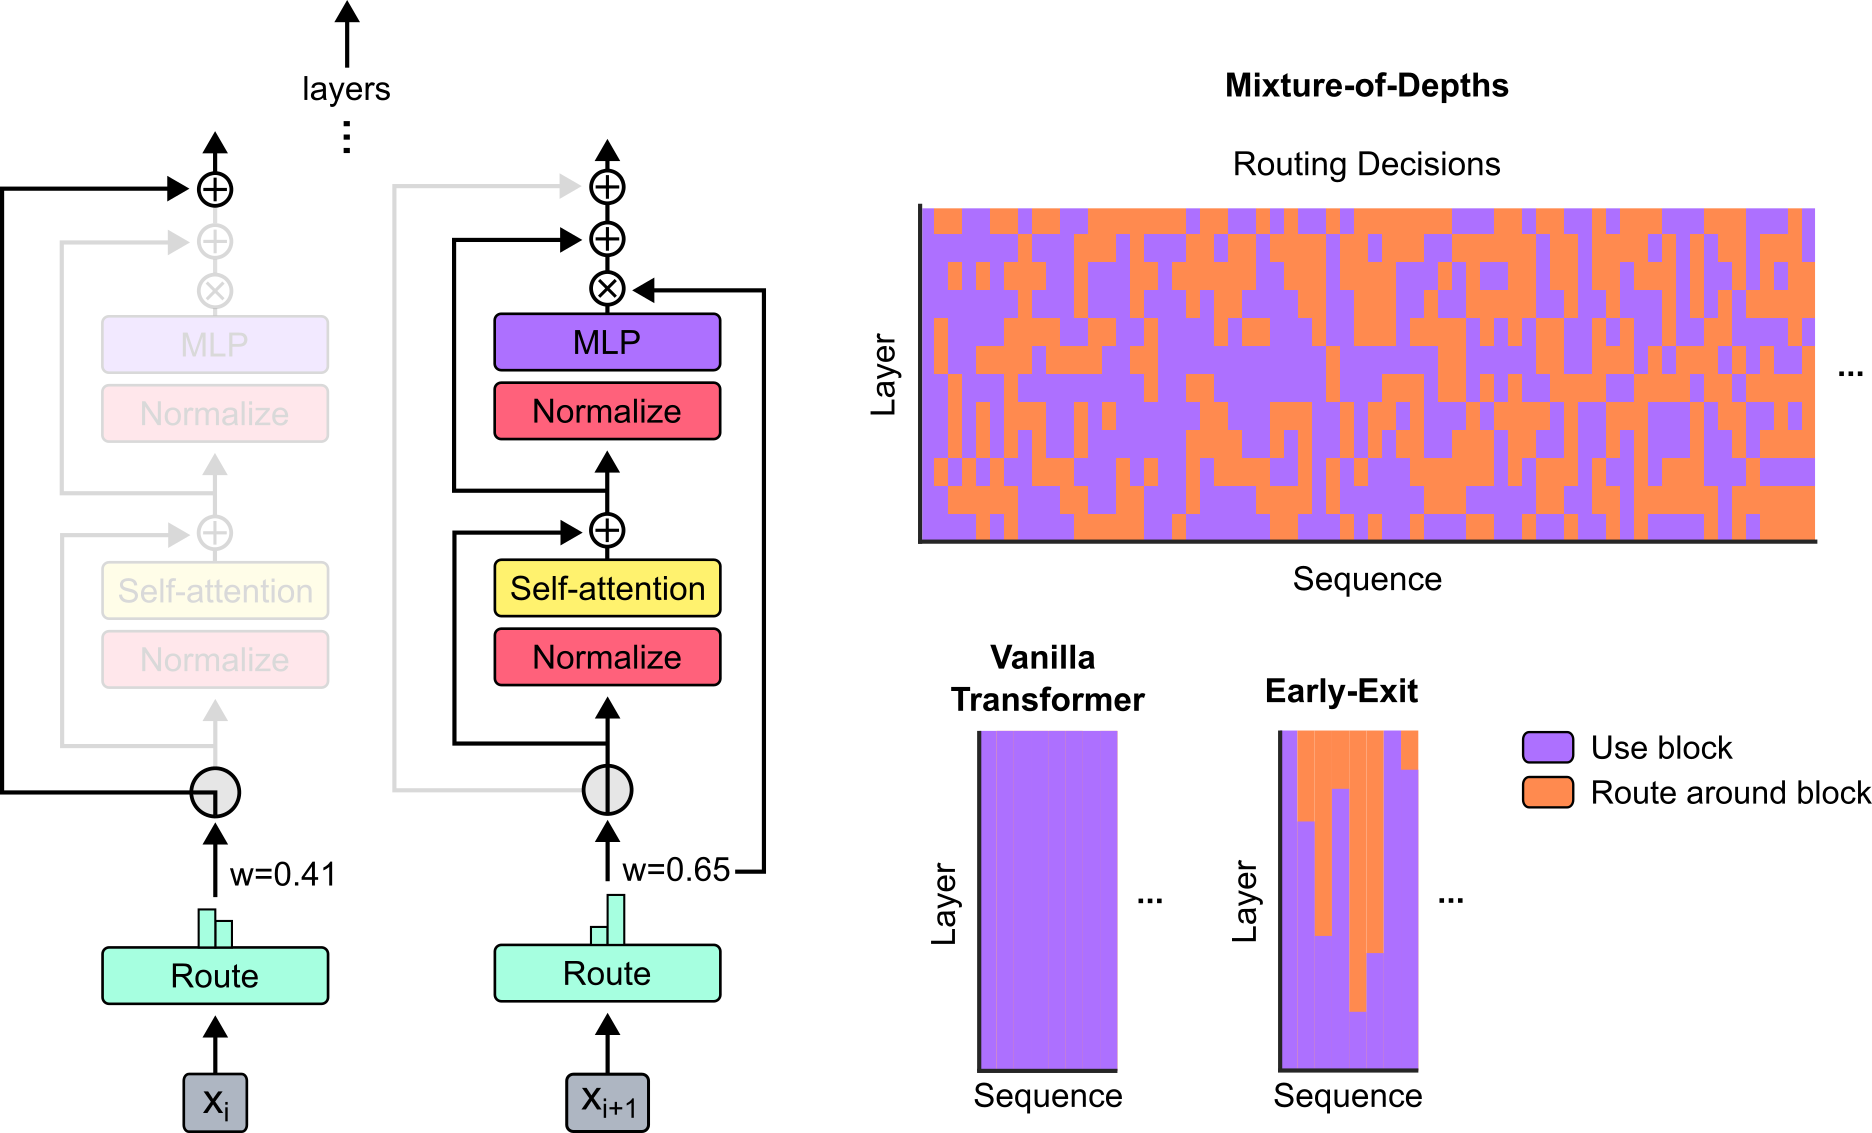
\includegraphics[width=0.95\textwidth]{mod.png}
\caption{\textbf{محول مزيج الأعماق.} كما هو الحال في محولات مزيج الخبراء (MoE)، نستخدم موجهًا للاختيار من بين المسارات الحسابية المحتملة. لكن على عكس محولات MoE، تكون الخيارات المحتملة هي حساب كتلة قياسية (أي الانتباه الذاتي وMLP) أو اتصال متبقٍ. نظرًا لأن بعض الرموز المميزة تأخذ هذا المسار الثاني، فإن محولات مزيج الأعماق (MoD) لها بصمة إجمالية أصغر من FLOP مقارنةً بالمحولات العادية أو MoE. في أعلى اليمين، تم تصوير قرارات توجيه نموذج مدرب لتسلسل قصير تم اقتطاعه إلى 64 رمزًا مميزًا لأغراض التصور. عند فحص الخيارات، يمكن للمرء أن يجد رموزًا مميزة تتم معالجتها بواسطة طبقات الكتل اللاحقة، على الرغم من المرور عبر عدد قليل نسبيًا من الكتل الإجمالية خلال عمق النموذج. هذه ميزة فريدة من MoD مقارنة بالحوسبة الشرطية التقليدية القائمة على التوقف، أو المحولات "الخروج المبكر" أو العادية، والتي تشارك الكتل بالتسلسل بدلاً من ذلك أو تشارك كل كتلة.}
\label{fig:mixture-of-depths}
\end{figure}

\section{الخلفية}
أصبحت بنية المحول هي محرك الثورة في الذكاء الاصطناعي العملي، مما أدى إلى قدرات غير مسبوقة بتكلفة عمليات التدريب والخدمة المكلفة. وقد أثار هذا اهتمامًا هائلاً بجعل بنية المحول أكثر كفاءة \citep{tay_efficient, gupta2021compression}. أحد الأساليب الواعدة هو \textit{الحوسبة الشرطية}، حيث تحدد الآليات المتعلمة متى وكيف يتم إنفاق الحساب. تم تقديم هذا المصطلح من قبل \citet{bengio2013deep}، وتم استكشاف المفهوم بمزيد من التفصيل على مدى السنوات القليلة التالية \citep{bengio2013estimating, cho2014exponentially, graves_adaptive, jernite2017variable, bengio2016conditional, wang_skipnet}.

طورت مجموعة واسعة من الأعمال الحديثة طرقًا للحساب الشرطي للمحولات. يركز بعض هذا العمل على "الخروج المبكر"، أي التعلم لتحديد متى يجب إنهاء الحساب على رمز معين، مما يسمح للرمز بتخطي أي طبقات محول متبقية بعد اتخاذ قرار الخروج \citep{elbayad_depth, liu2021anytime, schuster2022confident}. في MoD، على عكس أساليب الخروج المبكر، يمكن للرمز تخطي الطبقات الوسطى، ثم يتم تحديثه عبر الانتباه الذاتي مع الرموز التي مرت عبر جميع الطبقات الوسطى. نعتقد أن هذه قد تكون خاصية مفيدة.

طور عمل آخر أساليب لتكرار طبقات المحول مع أوزان مشتركة لعدد من الخطوات التكيفية \citep{simoulin-crabbe-2021-many, dehghani2018universal}. طور \citep{bolya2023token} طريقة لاختيار الرموز لدمجها عند تشغيل الاستدلال على محول رؤية مدرب، والذي لا يتطلب أي تعلم بشكل ملحوظ. يستخدم \citet{lei2023conditional} الحساب الشرطي في إعداد الضبط الدقيق من خلال البناء على نهج المحول \citep{he2021towards} لتعلم تخطي كتل الأوزان المدربة مسبقًا المجمدة لصالح تشغيل محول مضبوط بدقة صغير فقط.

يستخدم CoLT5 \citep{ainslie2023colt5} التوجيه الشرطي لتحديد ما إذا كان رمز معين سيمر عبر مسار ثقيل أو خفيف لكل طبقة أمامية. علاوة على ذلك، يستخدمون آلية التوجيه نفسها لتحديد ما إذا كان الرمز سيحضر جميع الرموز الأخرى أو عدد قليل مختار، كما في \citet{guo2022longt5}. مثل MoD، يستخدم CoLT5 القيمة الأعلى k الناعمة لاتخاذ قرارات التوجيه. ومع ذلك، يركز CoLT5 على إعداد التشفير والتفكيك، وبالتالي لا يحتاج إلى التصدي لمشكلة فك التشفير المتسلسل الفعال بالنظر إلى الطبيعة غير السببية لعملية top-k. في المقابل، يركز عملنا الحالي مع MoD على إعداد فك التشفير فقط، لذلك نقترح موجهًا تنبؤيًا لتمكين الاستدلال الفعال للحوسبة الشرطية في المحولات.

أحد الصياغات الناجحة للحوسبة الشرطية هي طبقة "خليط الخبراء" (MoE) كما قدمها \citet{shazeer2017outrageously}. تم تطويره في البداية في سياق LSTMs، وأظهرت الأعمال اللاحقة نتائج تجريبية مقنعة لـ MoE مع المحولات \citep{lepikhin2020gshard, fedus2022switch, zoph2022stmoe}. على عكس نهج الحساب الشرطي الأخرى التي تحاول الحفاظ على الحساب أو إنفاقه إضافيًا، تستخدم محولات MoE منطق شرطي لتوجيه الرموز إلى إحدى MLPs الخبيرة العديدة مع الحفاظ على إجمالي إنفاق الحساب ثابتًا. يمكن اعتبار طريقة مزيج الأعماق الخاصة بنا على أنها تستخدم منطق التوجيه من محولات MoE، ولكن بدلاً من وجود خبراء متعددين، تنشر MoD خبيرًا واحدًا يمكن تخطيه ديناميكيًا.

\section{تنفيذ محولات مزيج الأعماق}
استراتيجيتنا العامة هي كما يلي:
\begin{itemize}
\item تعيين ميزانية حوسبة ثابتة تكون أقل من تلك الخاصة بمحول عادي مكافئ عن طريق تحديد عدد الرموز في تسلسل يمكنها المشاركة في حسابات الكتلة (أي الانتباه الذاتي و MLP اللاحق). على سبيل المثال، بينما قد يسمح محول عادي لجميع الرموز في التسلسل بالمشاركة في الانتباه الذاتي، قد نحد من العدد إلى 50٪ من الرموز في التسلسل. انظر القسم \ref{sec:define-compute-budget}.
\item استخدام موجه لكل كتلة لإصدار وزن قياسي لكل رمز، والذي يعبر عن تفضيل الموجه لهذا الرمز للمشاركة في حسابات الكتلة أو تجاوزها. انظر القسم \ref{sec:routing-to-nowhere}.
\item تحديد أوزان القياس العلوية $k$ (لكل تسلسل، لكل كتلة) لتحديد تلك الرموز التي ستشارك في حسابات الكتلة. نظرًا لأن $k$ رموز ستشارك بالضبط في حسابات الكتلة، يظل الرسم البياني للحساب وأحجام المصفوفة ثابتة طوال التدريب؛ إنها مجرد مشاركة الرموز التي تكون ديناميكية وحساسة للسياق، كما يحددها الموجه. انظر القسم \ref{sec:routing-scheme}.
\end{itemize}

ثم نناقش بعض التعقيدات عند أخذ العينات بعد التدريب في القسم \ref{sec:sampling}.

\subsection{تحديد ميزانية الحوسبة}
\label{sec:define-compute-budget}

لفرض إجمالي ميزانية الحوسبة لكل تمرير أمامي، نستفيد من مفهوم \textbf{السعة}، والذي يحدد العدد الإجمالي للرموز التي تشكل إدخال حساب معين (على سبيل المثال، الرموز التي تشارك في الانتباه الذاتي، خبير معين في محولات MoE ، إلخ). على سبيل المثال، يحتوي الانتباه الذاتي و MLP في كل كتلة محول عادية على سعة تبلغ $T$---العدد الإجمالي للرموز عبر التسلسل والدفعة. من ناحية أخرى، تستخدم محولات MoE سعة أقل من $T$ لكل خبير MLP من أجل تقسيم الحساب الإجمالي بشكل أكثر تساويًا بين كل خبير. ولكن، نظرًا لأنها تستخدم خبراء متعددين لكل كتلة، فإن سعتها الإجمالية تقريبًا مساوية لتلك الخاصة بمحول افتراضي.

بشكل عام، سعة الرمز هي التي تحدد إجمالي عدد FLOPs للمحولات التي تستخدم الحوسبة الشرطية، بدلاً من نتائج أي قرارات توجيه. هذا لأن التنفيذات ذات الرسم البياني الثابت تأخذ في الاعتبار أسوأ السيناريوهات؛ على سبيل المثال، سيتم حشو مدخلات الحساب بمقدار سعتها حتى إذا انتهى الأمر بتوجيه عدد قليل نسبيًا من الرموز إليها، و/أو سيتم إسقاط الرموز من الحساب إذا تم تجاوز السعة.

يمكننا تحقيق هدفنا المتمثل في استخدام ميزانية حوسبة أصغر لكل تمرير إلى الأمام مقارنة بمحول قياسي عن طريق تقليل سعة الحسابات. ومع ذلك، فإن استخدام ميزانية حوسبة أصغر بشكل عشوائي سيؤدي إلى تدهور الأداء. نفترض أن \textit{بعض} الرموز قد لا تتطلب الكثير من المعالجة مثل الآخرين، ويمكن تحديد هذه الرموز من خلال التعلم. لذلك، إذا تعلمت الشبكة اختيار الرموز الصحيحة لملء سعاتها، فقد تحافظ على أدائها. في ما يلي نصف مخططات التوجيه التي يمكن استخدامها لهذا الغرض.

\subsection{التوجيه حول كتل المحولات}
\label{sec:routing-to-nowhere}
نأخذ في الاعتبار الإعداد الذي نوجه فيه الرموز إلى أحد المسارين الحسابيين: (1) كتل الانتباه الذاتي و MLP، و (2) اتصال متبقي. الأخير رخيص من الناحية الحسابية، وينتج عنه إخراج كتلة يتم تحديده بالكامل من خلال قيمة إدخاله. المسار الأول مكلف من الناحية الحسابية.

سيكون إجمالي عدد FLOPs لكل تمرير أمامي أقل من ذلك في محول افتراضي إذا قمنا بتعيين السعة للمسار (1) على أي شيء أقل من $T$ (إجمالي عدد الرموز عبر التسلسل والدفعة). على سبيل المثال، إذا قمنا بتعيين سعة الكتلة على $\frac{T}{2}$ (أي نصف عدد الرموز كما هو الحال في محول افتراضي)، فإن ضرب المصفوفة الاستعلام في المفتاح أثناء الانتباه الذاتي يصبح 25 ٪ مكثفًا لـ FLOP مثل محول افتراضي ($(\frac{T}{2})^2$ مقابل $T^2$). يمكن لحسابات مماثلة تحديد وفورات FLOP لـ MLP.

بشكل حدسي، ينخفض إجمالي FLOPs لكل تمرير أمامي (وينخفض الوقت اللازم لإكمال التمرير الأمامي) بالتناسب مع مدى عدوانية تقليص سعات الكتل. ومع ذلك، سيتأثر الأداء اللاحق أيضًا بمدى عدوانية تقليص سعات الكتل، وخوارزمية التوجيه التي ننفذها.

في أحد الأطراف، إذا تركنا سعة كل كتلة عند $T$ ووجهنا كل رمز إلى (بدلاً من \emph{حول}) كل كتلة، فإننا نستعيد محولاً افتراضيًا. في الطرف الآخر، إذا قمنا بتعيين سعة كل كتلة على $0$ وتوجيه جميع الرموز \emph{حول} كل كتلة، فسنبقى مع نموذج سريع جدًا لا يتفاعل مع الغالبية العظمى من معلمات

المحول، ولا شك أن لديه أداءً سيئًا لاحقًا. نفترض أنه في مكان ما بين هذين الطرفين يوجد نموذج أمثل أسرع من محول افتراضي ويعمل بشكل جيد، إن لم يكن أفضل، وفي الوقت نفسه يكون أسرع في الخطوة.

\subsection{مخططات التوجيه}
\label{sec:routing-scheme}
بسذاجة، يمكن للمرء الاستفادة من العشوائية لتوجيه الرموز، أسوةً بـ "فقدان" الطبقة أو الكتلة. نقدم مخطط التوجيه هذا كتحكم، وسنظهر أنه يقل أداؤه بشكل كبير مقارنة بالمحولات الأساسية.

نفترض أن التوجيه \emph{المتعلم} أفضل. بشكل حدسي، يجب أن تكون الشبكة قادرة على تعلم الرموز التي تتطلب معالجة أكثر أو أقل من غيرها. إذا كنا على صواب في أن المحولات غالبًا ما تنفق حسابات أكثر مما تحتاجه لتقديم تنبؤاتها، فإنها مسألة تجريبية لمعرفة مدى عدوانية يمكننا تقليص سعة كل كتلة، وبالتالي، عدد الرموز التي يمكننا تحمل توجيهها حول كل كتلة.

\begin{figure}[h]
\centering
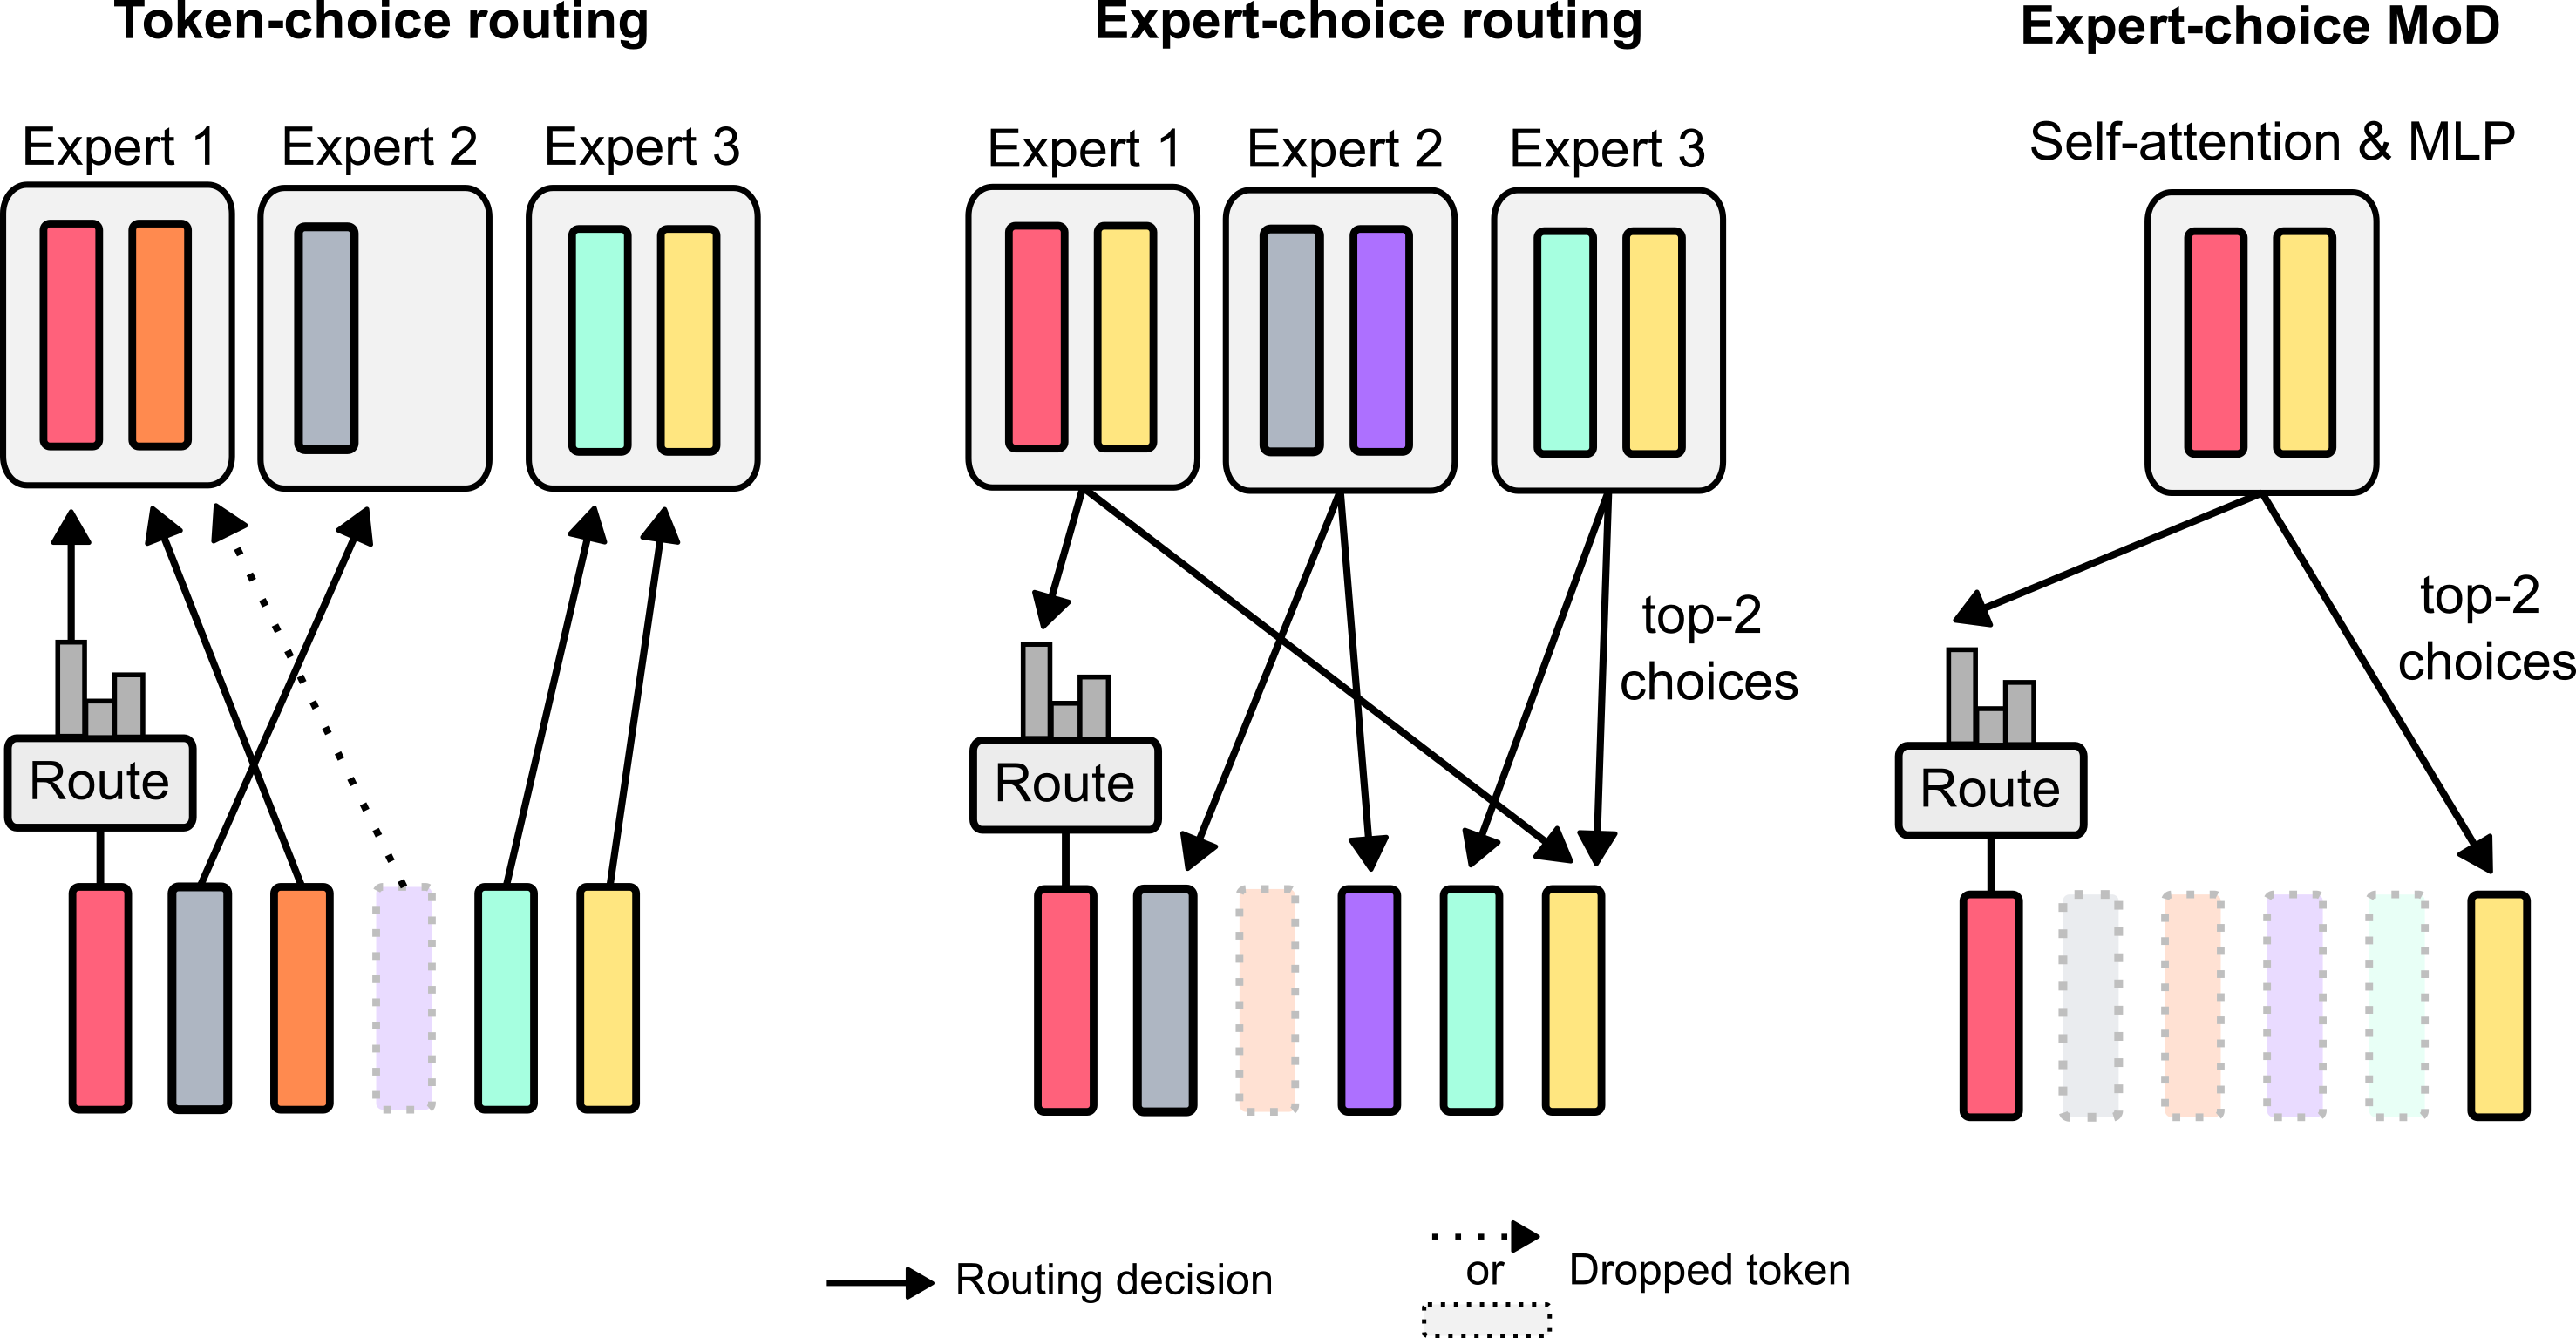
\includegraphics{routing.png}
\caption{\textbf{مخططات التوجيه.} يتم توجيه الرموز إلى مسار الحساب الذي تختاره عند استخدام التوجيه المعتمد على اختيار الرمز (يسار). إذا تجاوز مسار معين سعته (على سبيل المثال، أكثر من رمزين في هذا المثال)، فيجب إسقاط الرموز الفائضة (الرمز الأرجواني). يعتمد الرمز الدقيق الذي يتم إسقاطه في النهاية على التنفيذ الدقيق في الكود الأساسي. على سبيل المثال، غالبًا ما تُعطى الأولوية للرموز التي تأتي في وقت سابق في تسلسل أو ترتيب الدفعة. باستخدام التوجيه المعتمد على اختيار الخبير (وسط)، يتم اختيار $k$ رمز بالضبط (في هذه الحالة، اثنان) لكل مسار باستخدام آلية أعلى $k$ عبر أوزان موجه الرموز. هنا، يتم إسقاط الرموز إذا لم تكن من بين أعلى $k$ فيما يتعلق بأي مسار معين (الرمز البرتقالي)، وقد يتم توجيه بعض الرموز حتى إلى مسارات متعددة (الرمز الأصفر). في هذا العمل ننشر التوجيه المعتمد على اختيار الخبير (يمين). ومع ذلك، لأننا نستخدم مسارًا واحدًا فقط، فإننا \emph{نستفيد} من المعرفة الضمنية بأنه سيتم إسقاط الرموز إذا كان $k$ أقل من طول التسلسل حتى نتمكن من توجيه الرموز بعيدًا عن حسابات الانتباه الذاتي و MLP، وبالتالي إنفاق عدد أقل من FLOPs في تمرير أمامي معين للنموذج.}
\label{fig:routing}
\end{figure}

هناك مخططان متعلمان للتوجيه نأخذهما في الاعتبار  : اختيار الرمز واختيار الخبير. في التوجيه المعتمد على اختيار الرمز، ينتج الموجه توزيعات احتمالية لكل رمز عبر المسارات الحسابية (على سبيل المثال، عبر هويات الخبراء في محولات MoE). ثم يتم نقل الرموز إلى المسار الذي تفضله --- أي ذلك الذي يحتوي على أعلى احتمال --- وتضمن الخسائر المساعدة عدم تقارب جميع الرموز إلى نفس المسار. يمكن أن يواجه التوجيه المعتمد على اختيار الرمز مشاكل في موازنة الحمل لأنه لا يوجد ضمان بأن الرموز تقسم نفسها بشكل مناسب بين المسارات الممكنة. يقلب "التوجيه المعتمد على اختيار الخبير" هذه الوصفة رأسًا على عقب: بدلاً من أن تختار الرموز المسار الذي تفضله، يختار كل مسار بدلاً من ذلك أعلى $k$ رموز بناءً على تفضيلات الرموز. هذا يضمن توازن حمل مثالي لأن $k$ رموز مضمونة ليتم نقلها إلى كل مسار. ومع ذلك، قد يؤدي ذلك إلى معالجة زائدة أو غير كافية لبعض الرموز، لأن بعض الرموز قد تكون من بين أعلى $k$ لمسارات متعددة، أو لا شيء منها.

قررنا الاستفادة من التوجيه المعتمد على اختيار الخبير لعدة أسباب. أولاً، إنه يتجنب الحاجة إلى خسارة موازنة مساعدة. ثانيًا، نظرًا لأن عملية أعلى $k$ تعتمد على حجم أوزان الموجه، فإن مخطط التوجيه هذا يسمح لأوزان التوجيه النسبية بالمساعدة في تحديد الرموز الأكثر احتياجًا لحسابات الكتلة؛ يمكن للموجهات محاولة \emph{ضمان} أن تكون الرموز الأكثر أهمية من بين أعلى $k$ عن طريق تعيين وزنها بشكل مناسب، وهو أمر غير ممكن مع مخططات التوجيه المعتمدة على اختيار الرمز. بالنسبة لحالة الاستخدام المحددة الخاصة بنا، حيث يكون أحد المسارات الحسابية عملية فارغة بشكل أساسي، قد يكون من الضروري توجيه الرموز المهمة بعيدًا عن العملية الفارغة. ثالثًا، لأننا نوجه فقط عبر مسارين، يمكن لعملية أعلى $k$ واحدة أن تقسم الرموز بكفاءة إلى مجموعتين متبادلتين، واحدة لكل مسار حسابي، مما يمنع مشكلة المعالجة الزائدة أو غير الكافية المذكورة أعلاه.

\subsection{تنفيذ التوجيه}
\label{sec:routing-implementation}
كتذكير بالحدس رفيع المستوى، تتم معالجة كل رمز بواسطة موجه لإنتاج وزن قياسي، ثم يتم استخدام أعلى $k$ أوزان لاختيار هويات الرمز التي ستوجه من خلال كتلة محول، والتي تشمل الانتباه الذاتي و MLP اللاحق.

لنفترض أن لدينا مجموعة من تضمينات الرموز في تسلسل بطول $S$ لطبقة معينة $l$؛ أي $X^l = {x_i^l | i \text{ عدد صحيح، }1 \leq i \leq S }$. وزن الموجه لرمز معين هو قيمة قياسية تنتج نتيجة إسقاط خطي، $r_i^l=w_\theta^Tx_i^l$.

هدفنا هو استخدام أوزان الموجه هذه لتحديد ناتج حساب كتلة كل رمز. لنفترض $P_\beta(R^l)$ هو المئوي $\beta$ لمجموعة أوزان الموجه $R^l$، حيث $\beta=1 - C/S$ و $C$ هو سعة محددة من قبل المستخدم لكل عنصر دُفعة (عدد صحيح $<S$ يحدد عدد الرموز من تسلسل سيتم معالجته بواسطة دالة معينة). ناتج كتلة لرمز معين هو:



هنا، $\tilde{X}^l$ هي مجموعة الرموز التي تكون قيمها $r_i^l > P_\beta(R^l)$ (أي الرموز "الأعلى-k")، و $f$ تشمل الانتباه الذاتي و MLP اللاحق. لاحظ أن الناتج لرمز معين $x_i^{l+1}$ قد يعتمد على رموز أخرى $x_{i \neq j}^l$ بسبب عملية الانتباه الذاتي. إن عدد العناصر في $\tilde{X}^l$ هو $C$ (أو $k$): السعة المحددة من قبل المستخدم. لذلك، يحقق محول مزيج الأعماق وفورات في الحساب مقارنة بالأساسي لأن الإدخال لحسابات الكتلة $f$ يشمل عددًا أقل من الرموز من المعتاد ($C < S$)، مما يجعل الانتباه الذاتي و MLP أقل تكلفة.

من الجدير بالذكر أننا نضرب ناتج الدالة $f$ في أوزان الموجه. هذا يضع أوزان الموجه على طول "مسار التدرج"، وبالتالي يخضعها لقوى النزول التدريجي خلال مسار مهمة نمذجة اللغة (قمنا بتجربة إصدارات حيث يتم تضمين أوزان الموجه أيضًا على طول المسار الحسابي لتلك الرموز التي تتجاوز حسابات الكتلة، ولكن يبدو من الكافي --- وأبسط من الناحية التنفيذية --- تضمين أوزان الموجه فقط على طول المسار الحسابي لتلك الرموز التي لا تتجاوز حسابات الكتلة).

\subsection{أخذ العينات}
\label{sec:sampling}
بينما يتمتع التوجيه المعتمد على اختيار الخبير بعدد من المزايا، إلا أن له مشكلة واحدة مميزة: عملية أعلى $k$ غير سببية. هذا يعني أن ما إذا كان وزن توجيه رمز معين من بين أعلى $k$ للتسلسل يعتمد على قيم أوزان التوجيه للرموز التي تأتي بعده، والتي لا نستطيع الوصول إليها عند أخذ العينات بشكل تراجعي.

اختبرنا طريقتين للتغلب على هذه المشكلة. الأولى تقدم خسارة بسيطة مساعدة تؤثر تجريبيًا على الهدف الأساسي لنمذجة اللغة بنسبة 0.2-0.3٪ تقريبًا، ولكنها تسمح لنا بأخذ العينات من النموذج بشكل تراجعي. نستخدم خسارة إنتروبيا متقاطعة ثنائية حيث توفر مخرجات الموجه اللوجيتات، وتوفر اختيارات أعلى $k$ لهذه اللوجيتات الأهداف (أي 1 إذا كان الرمز من بين أعلى $k$، و 0 إذا لم يكن). بشكل حدسي، تركز هذه الخسارة دالة سيجموي

د لمخرجات الموجه حول 0.5؛ تتعرض الرموز التي يتم اختيارها من بين أعلى k للضغط لإنتاج مخرجات موجه أعلى من 0.5، وتتعرض تلك التي ليست من بين أعلى k للضغط لإنتاج مخرجات موجه أقل من 0.5. تقدم الطريقة الثانية مُنشئ MLP مساعد صغير (يشبه موجهًا ثانيًا) يتلقى نفس مدخلات الموجه (مع إيقاف التدرج)، ولكن مخرجاته هي تنبؤ بما إذا كان هذا الرمز سيكون من بين أعلى k أم لا في التسلسل. لا تؤثر هذه الطريقة على هدف نمذجة اللغة، وتجريبيًا لا تؤثر بشكل كبير على سرعة الخطوة.

مع هاتين الطريقتين الجديدتين، يمكننا أخذ العينات بشكل تراجعي عن طريق اختيار توجيه الرموز \textit{إلى} أو \textit{تجاوز} الكتلة بناءً على مخرجات الموجه، والتي لا تعتمد على أي معلومات من الرموز المستقبلية. نقدم دليلاً تجريبيًا على أن هذه مهمة مساعدة سهلة نسبيًا تصل بسرعة إلى دقة 99٪.

\subsection{طرق التدريب}
تستخدم جميع النماذج نفس التكوينات الأساسية لمعلمات النظام (على سبيل المثال، جداول جيب التمام المساوية لـ 1 × خطوات التدريب، حجم دفعة 128، طول تسلسل 2048) باستثناء التغييرات في عدد الطبقات والرؤوس وحجم التضمين لإنتاج نماذج بأحجام مختلفة أثناء تحليلات isoFLOP.

\section{النتائج}
\subsection{التدريب ومقارنات isoFLOP}
\begin{figure}[h]
\centering
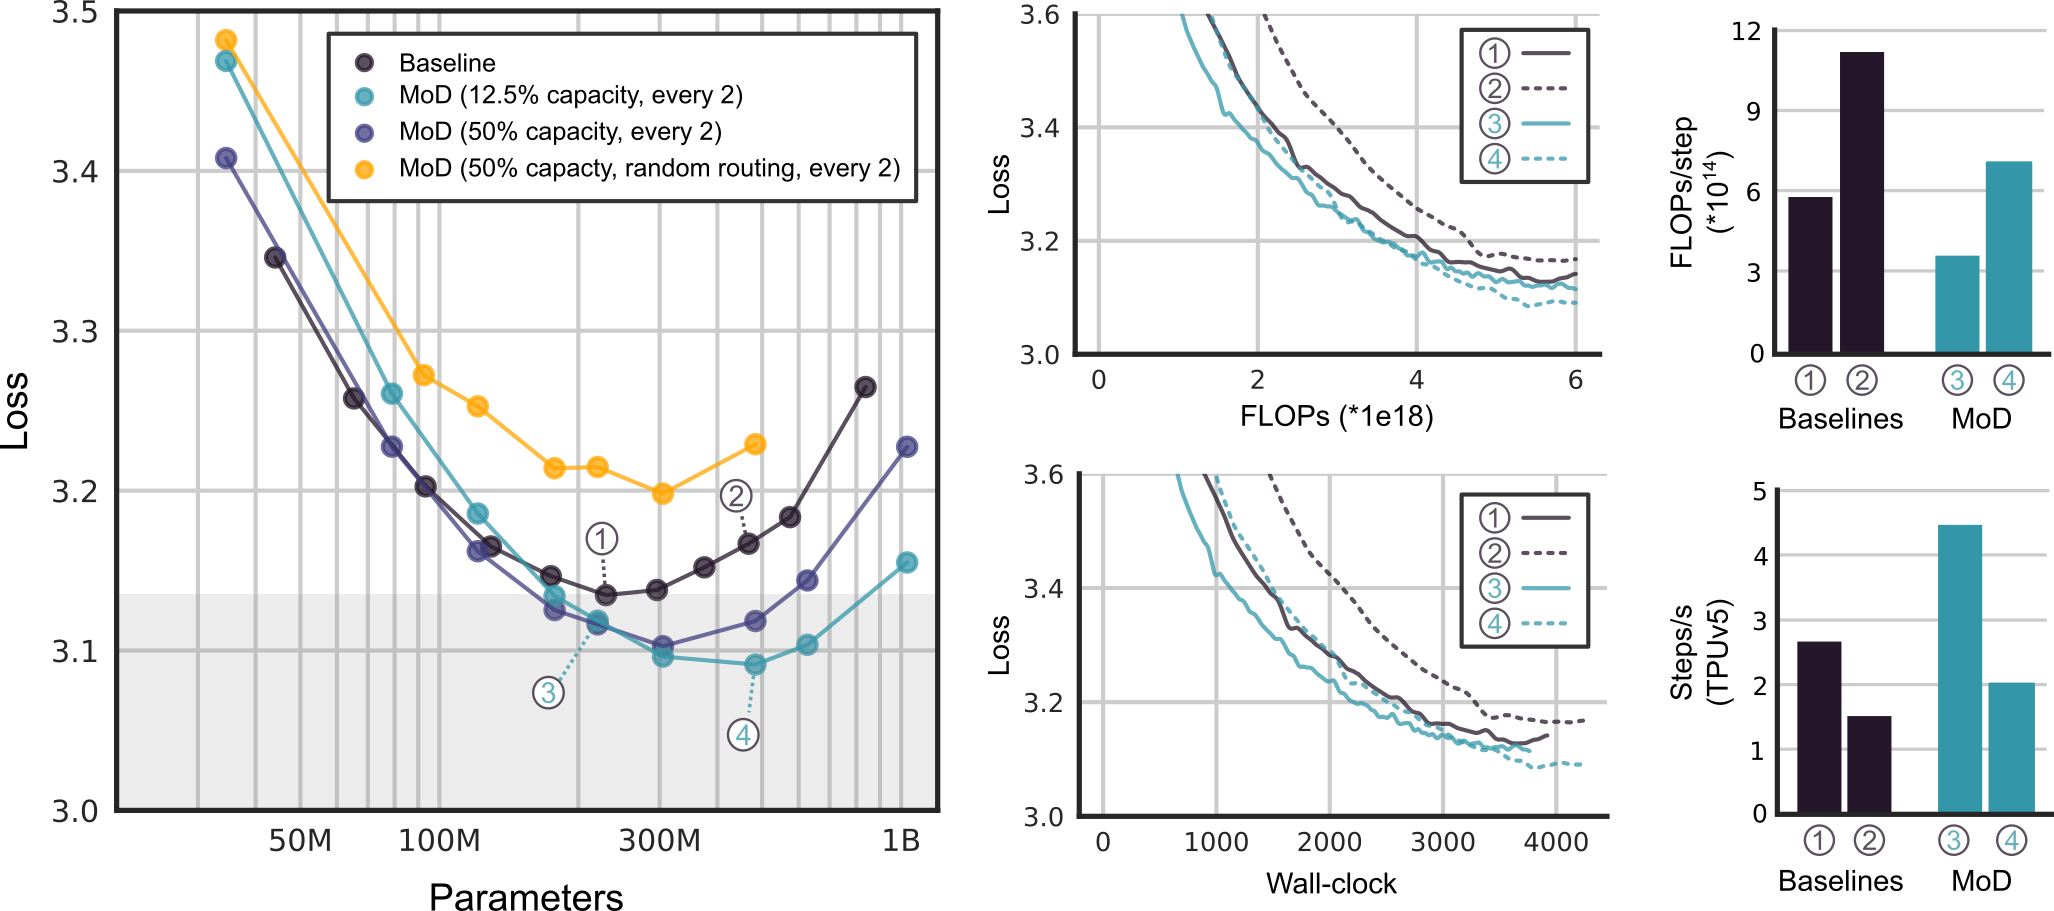
\includegraphics[width=\textwidth]{results-1.png}
\caption{\textbf{ضبط معلمات النظام لـ MoD.} تم تدريب نماذج متنوعة من محول MoD لمدة 6e18 FLOP لتحديد المعلمات المثلى للتحليلات اللاحقة لـ isoFLOP. في الرسم البياني الأيسر، يشير المربع الرمادي إلى النماذج التي تؤدي أداءً أفضل من أساس isoFLOP الأمثل. وجدنا أن أفضل نسخة من MoD هي تلك التي لديها خيار توجيه كل كتلة أخرى، والتي تستخدم أعلى k بقيمة 256 (لذلك، يتم معالجة 256 أو 12.5٪ من رموز التسلسل بواسطة الانتباه الذاتي و MLP اللاحق، بينما يتم توجيه 1792 رمزًا أو 87.5٪ من رموز التسلسل \emph{حول} الكتلة). يظهر على اليمين منحنيات التعلم لمجموعة مختارة من النماذج. من الجدير بالذكر أن النموذج رقم 3 يحقق أداءً مساويًا لأساس isoFLOP الأمثل ولكنه يتقدم بسرعة 66٪، نظرًا لعدد أقل نسبيًا من FLOP المطلوبة لكل تمرير أمامي.}
\label{fig:mod-learning-curve}
\end{figure}

قمنا أولاً بتدريب نماذج بميزانية FLOP صغيرة نسبيًا (6e18) لتحديد المعلمات المثلى (انظر الشكل \ref{fig:mod-learning-curve}). بشكل عام، وجدنا أن محولات MoD تسحب منحنى أساس isoFLOP "لأسفل وإلى اليمين". أي أن محول MoD الأمثل يحقق خسارة أقل من الأساس الأمثل، وأيضًا لديه معلمات أكثر. نتيجة محظوظة لهذا التأثير هي وجود نماذج MoD أصغر، بينما لا تكون نفسها مثالية لـ isoFLOP لإعداد المعلمات الخاصة بها، إلا أنها مع ذلك تؤدي بشكل مساوٍ أو أفضل من النموذج الأساسي الأمثل مع كونها أسرع. على سبيل المثال، محول MoD بمعلمات 220 مليون (الشكل \ref{fig:mod-learning-curve} النموذج رقم 3) يتفوق قليلاً على الأساس الأمثل لـ isoFLOP (أيضًا 220 مليون، الشكل \ref{fig:mod-learning-curve} النموذج رقم 1)، ولكنه أسرع بنسبة تصل إلى 60٪ في الخطوة أثناء التدريب. الأهم من ذلك، عند تشغيلها على أجهزة مكافئة، تستغرق هاتان النسختان من النموذج نفس الوقت تقريبًا على الساعة الجدارية للتدريب (الشكل \ref{fig:mod-learning-curve}).

اختبرنا التوجيه لكل كتلة أو كل كتلة أخرى، باستخدام سعات من 12.5٪ إلى 95٪ من إجمالي التسلسل. بينما كان توجيه كل \textit{كتلة أخرى} ضروريًا لأداء قوي، وجدنا أن تقليل السعة بشكل عدواني كان الأفضل (تم ملاحظة تحسينات تدريجية عند تقليل السعة إلى 12.5٪ من إجمالي التسلسل، بما يقابل توجيه 87.5٪ من الرموز \textit{حول} الكتل، مع تدهور الأداء بعد هذه النقطة). لذلك، يبدو أن الشبكة قوية في مواجهة تخفيضات السعة الكبيرة طالما أن هناك فرصة متكررة لعمليات الانتباه الذاتي وحسابات MLP بكامل السعة.

التوجيه المتعلم أمر بالغ الأهمية، حيث تؤدي محولات MoD التي تستخدم التوجيه العشوائي (المنفذ باستخدام عملية أعلى $k$ على أوزان الموجه المعاينة من توزيع جاوسي) أداءً أسوأ بكثير من كل من الأساس و محول MoD العادي (الشكل \ref{fig:mod-learning-curve}).

\begin{figure}[h]
\centering
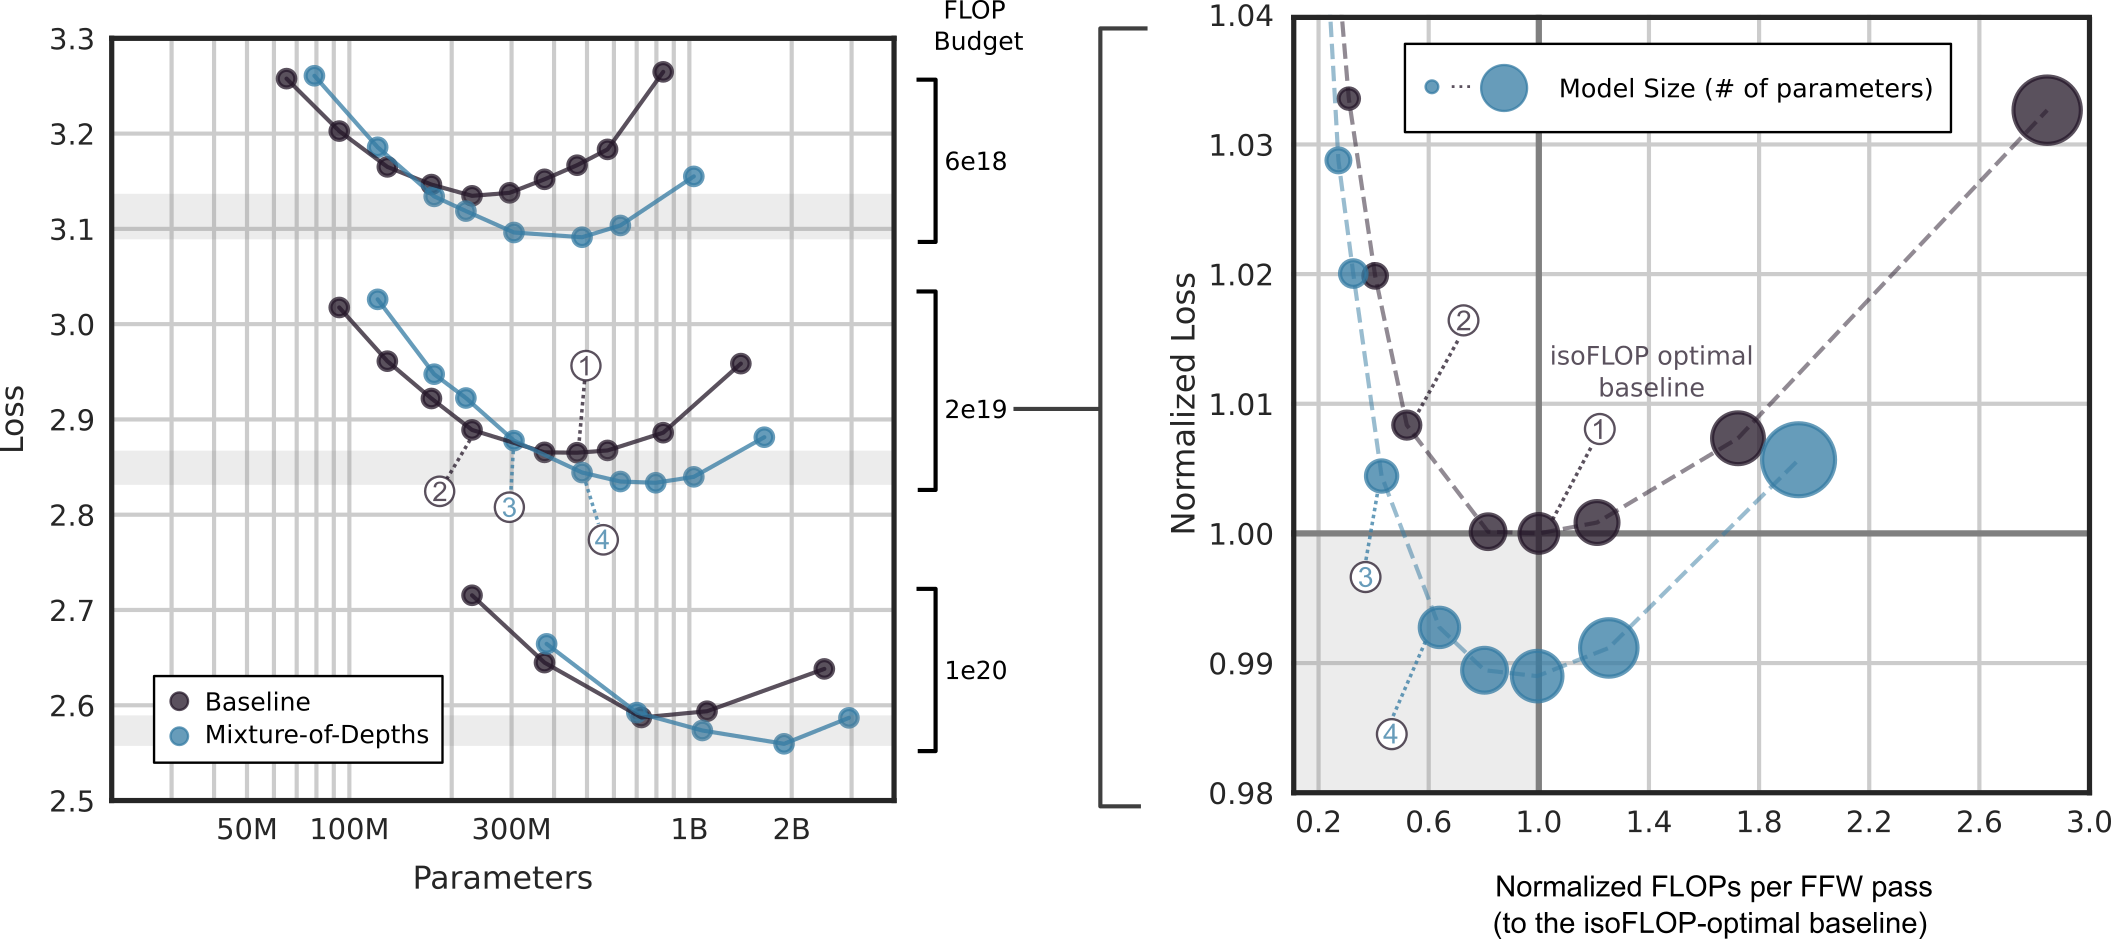
\includegraphics[width=\textwidth]{mod-isoflop.png}
\caption{\textbf{تحليل isoFLOP.} استخدمنا نسخة MoD بسعة 12.5٪ لإجراء تحليل isoFLOP لـ 6e18 و 2e19 و 1e20 FLOP، وتدريب نماذج تتراوح في الحجم من 60 مليون إلى 3 مليار معلمة. يظهر على اليمين FLOP النسبية لكل تمرير أمامي (تم تطبيعها على أساس isoFLOP الأمثل). توجد متغيرات MoD تكون أسرع في الخطوة (بحكم الحاجة إلى عدد أقل من FLOP لكل تمرير أمامي) وأداء أفضل من أساس isoFLOP الأمثل.}
\label{fig:isoflop}
\end{figure}

يوضح الشكل \ref{fig:isoflop} تحليل isoFLOP لإجمالي FLOP بقيمة 6e18 و 2e19 و 1e20. يستمر الاتجاه الذي تمتلك فيه محولات MoD الأمثل من حيث FLOP معلمات أكثر من الأساس لميزانيات FLOP الأكبر هذه. من الجدير بالذكر أنه توجد متغيرات MoD تقدر بشكل أسرع من الأساس الأمثل isoFLOP (تقاس بالخطوات في الثانية عند التدريب على أجهزة مكافئة) مع تحقيق خسارة أقل (في الشكل \ref{fig:isoflop} نصور FLOP المطبعة لكل تمرير أمامي بدلاً من وقت خطوة الساعة الجدارية \textit{per se}، ولكن من تجاربنا يرتبط الاثنان ارتباطًا وثيقًا. ويمكن إنتاج رسم بياني مماثل يُظهر أوقات خطوة الساعة الجدارية النسبية ويكون نفس الاتجاه الأساسي موجودًا).

تأتي مكاسب السرعة الخطوة من مصدرين. أولاً، نسبة FLOP لكل معلمة في محولات MoD أقل من الأساس لأن بعض نسبة من الرموز يتم توجيهها حول الكتل. لذلك، بالنسبة لحجم نموذج معين، يتطلب المحول عددًا أقل من FLOP لكل تمرير أمامي. ثانيًا، نظرًا لأن محولات MoD المثلى من حيث FLOP أكبر حجمًا وتحقق خسارة أقل من الأساس الأمثل isoFLOP، فهناك متغيرات MoD أصغر تؤدي بنفس الجودة أو أفضل من الأساس الأمثل isoFLOP، وهذه المتغيرات أسرع في الخطوة لأنها أصغر حجمًا. في المجمل، إذن، هناك محولات MoD تؤدي بنفس جودة خطوط الأساس المثلى isoFLOP وهي أسرع في الخطوة، سواء لأنها تستخدم عددًا أقل من FLOP لكل معلمة أو لأنها تستخدم عددًا أقل من المعلمات.

يكشف الشكل \ref{fig:isoflop} أيضًا عن نتيجة مهمة أخرى: محول MoD الأمثل هو الذي يستخدم عددًا من FLOP لكل تمرير أمامي مثل الأساس الأمثل isoFLOP. تسمح هذه النتيجة للمرء بالتنبؤ مباشرة بحجم محول MoD الذي سيعمل بشكل مثالي لميزانية تدريب isoFLOP معينة: يحتاج المرء فقط إلى ضبط حجم النموذج لتكوين MoD معين (أي السعة وتكرار التوجيه) لإنتاج نموذج يستخدم نفس عدد FLOP لكل تمرير أمامي مثل الأساس الأمثل isoFLOP، وسيكون لديهم متغير MoD الأمثل لهذا التكوين. تجريبيًا، نجد أنه من الأفضل إضافة العمق بدلاً من إضافة العرض عند إضافة FLOP إلى النموذج.

ومع ذلك، بينما يحدد FLOP لكل تمرير أمامي أي نموذج سيكون الأمثل isoFLOP، إلا أنه لا يتنبأ بما إذا كانت الخسارة المثلى ستتحسن عن الأساس (انظر الشكل \ref{fig:mod-learning-curve}. وتحديداً، يبدو أن السعة المثلى يمكن تحديدها تجريبيًا. وجدنا أنه من الأفضل استخدام كتل بسعة 12.5٪، كل كتلة أخرى.

لاحظنا أن محولات MoD حققت وفورات في الذاكرة مقارنة بالنماذج الأساسية المكافئة في الأحجام الأكبر، مع تطلب بعض المتغيرات عددًا أقل من الأجهزة الإجمالية (أي طوبولوجيا TPU أصغر). لم ندرس هذا بشكل مكثف، لكننا نتوقع أنه مع تطوير النماذج إلى أحجام أكبر، يمكن أن تكون هذه الوفورات اعتبارًا مهمًا عند اختيار متغيرات النموذج للتدريب، ويمكن أن يكون لها تأثيرات إيجابية كبيرة فيما يتعلق بحجم ذاكرة التخزين المؤقت KV أثناء أخذ العينات التراجعية.

\begin{figure}[h]
\centering
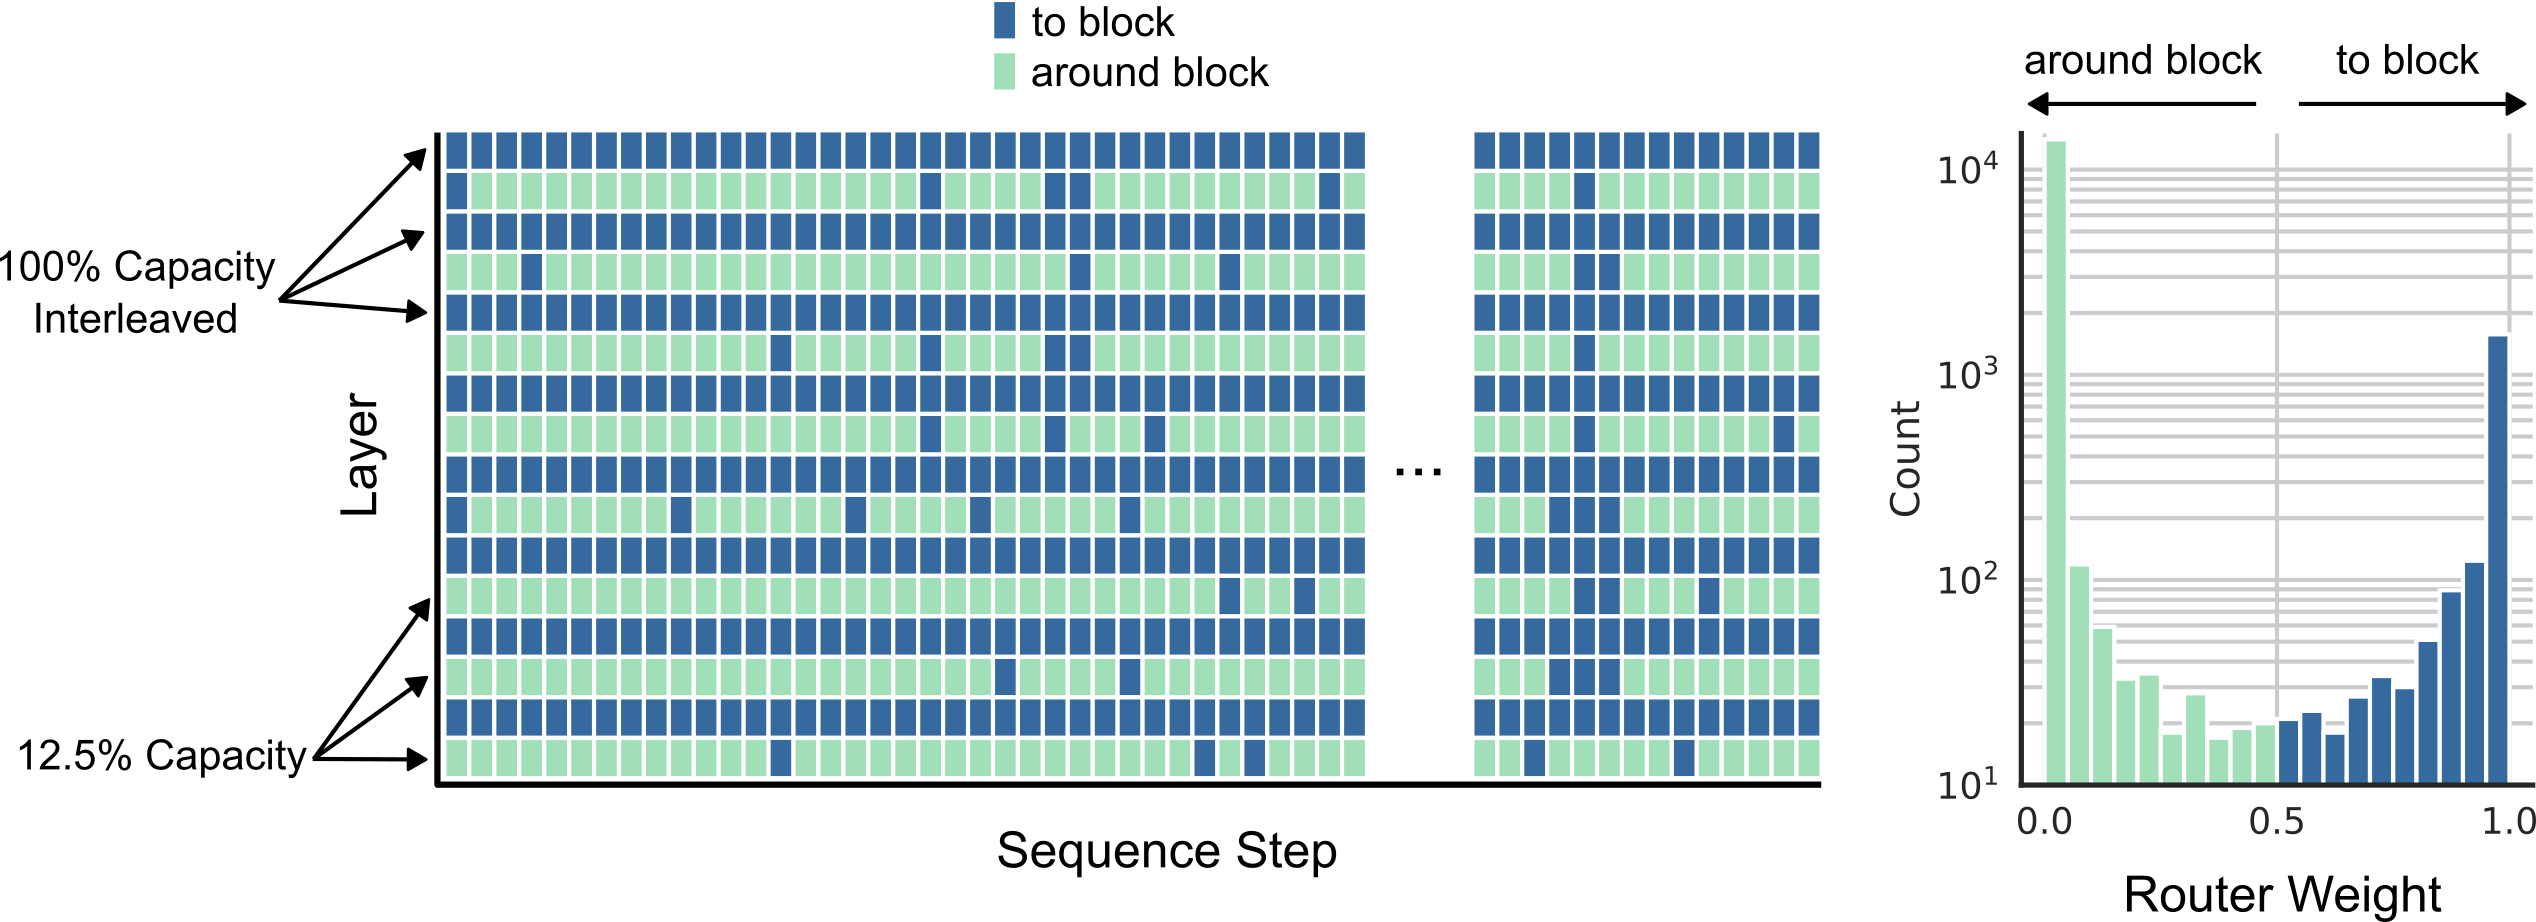
\includegraphics[width=\textwidth]{weight_analysis.png}
\caption{\textbf{تحليل التوجيه.} قمنا بتدريب محول MoD حيث تم إدراج كتل توجيه بنسبة 12.5٪ بين كتل الانتباه الكامل. كما هو متوقع، يكون عدد الرموز التي يتم توجيهها إلى (بدلاً من حول) الكتلة متناثرًا في كتل التوجيه، على الرغم من أن الشبكة تفضل أحيانًا توجيه رموز معينة إلى كل كتلة على طول عمقها. يمكن ملاحظة ذلك في الشكل الأيسر الذي يصور قرارات التوجيه، حيث نلاحظ شريطًا عموديًا من اللون الأزرق الداكن نحو نهاية التسلسل. كما هو متوقع، يكون توزيع أوزان الموجه كما يمليه الخسارة المساعدة: حوالي 12.5٪ من الأوزان أعلى من 0.5 و 87.5٪ أقل من ذلك (الرسم البياني، يمين).}
\label{fig:routing-analysis}
\end{figure}

يوضح الشكل \ref{fig:routing-analysis} قرارات التوجيه لمحول MoD تم تدريبه باستخدام كتل توجيه متداخلة. على الرغم من التوجيه العدواني حول الكتل، تتمكن المحولات من تحقيق تحسينات في الأداء مقارنة بخطوط الأساس. نلاحظ أنماطًا قد تستحق مزيدًا من الدراسة؛ وتحديدًا، تشارك بعض الرموز في كل كتلة على طول عمق المحول، بينما تقرر رموز أخرى التوجيه حول الكتل كلما أمكن ذلك. تشير التحليلات الأولية إلى أن الرموز التي تشارك في الكتل بشكل أكثر تواترًا ترتبط بتنبؤات الإخراج ذات الإنتروبيا الأعلى، والتي قد تتوافق مع التنبؤات التي يصعب إجراؤها.

\subsection{التقييم التراجعي}
\begin{figure}[h]
\centering
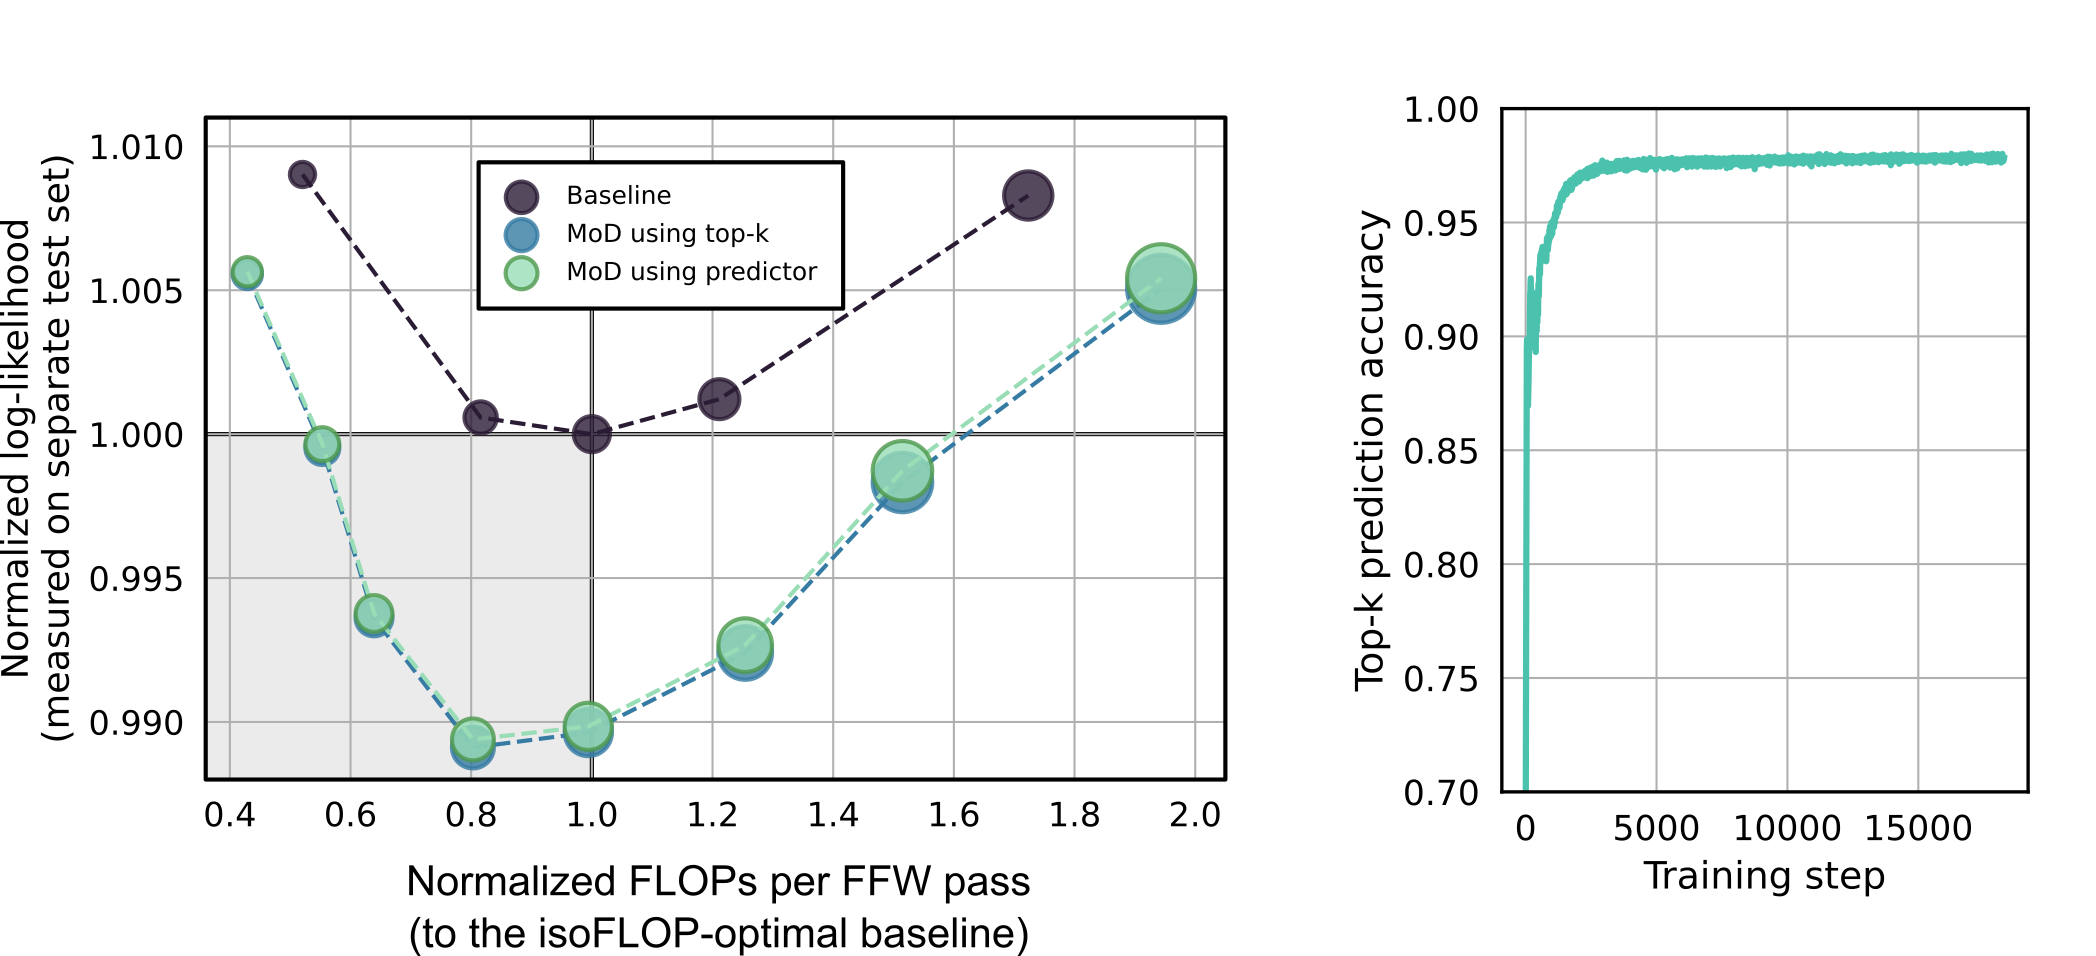
\includegraphics[width=\textwidth]{autoregressive.png}
\caption{\textbf{التقييم التراجعي.} يؤدي التبديل من مخطط التوجيه أعلى $k$ غير السببي في التدريب إلى نهج قائم على المنشئ السببي أثناء أخذ العينات التراجعية إلى تدهور أداء ضئيل. ربما يرجع ذلك إلى سهولة تعلم مشكلة التنبؤ هذه، والتي تصل إلى دقة 97٪ بسرعة في التدريب.}
\label{fig:autoregressive}
\end{figure}

قمنا بتقييم متغيرات MoD أثناء أخذ العينات التراجعية (انظر الشكل \ref{fig:autoregressive}). تم اختبار كل نموذج على نفس البيانات المحجوبة تمامًا والتي تتكون من 256000 تسلسل (500 مليون رمز). عند التبديل من طريقة التوجيه أعلى $k$ إلى طريقة التوجيه القائمة على المنشئ، لاحظنا تدهورًا ضئيلًا في الأداء. كما هو الحال في إعداد التدريب، هناك متغيرات MoD تؤدي أداءً أفضل من الأساس الأمثل isoFLOP، مع الحاجة إلى عدد أقل من FLOP لكل تمرير أمامي. تشير هذه النتائج إلى أن وفورات الحوسبة التي توفرها محولات MoD يجب أن تترجم إلى ما بعد إعداد التدريب.

\subsection{مزيج من الأعماق والخبراء (MoDE)}
\begin{figure}[h]
\centering
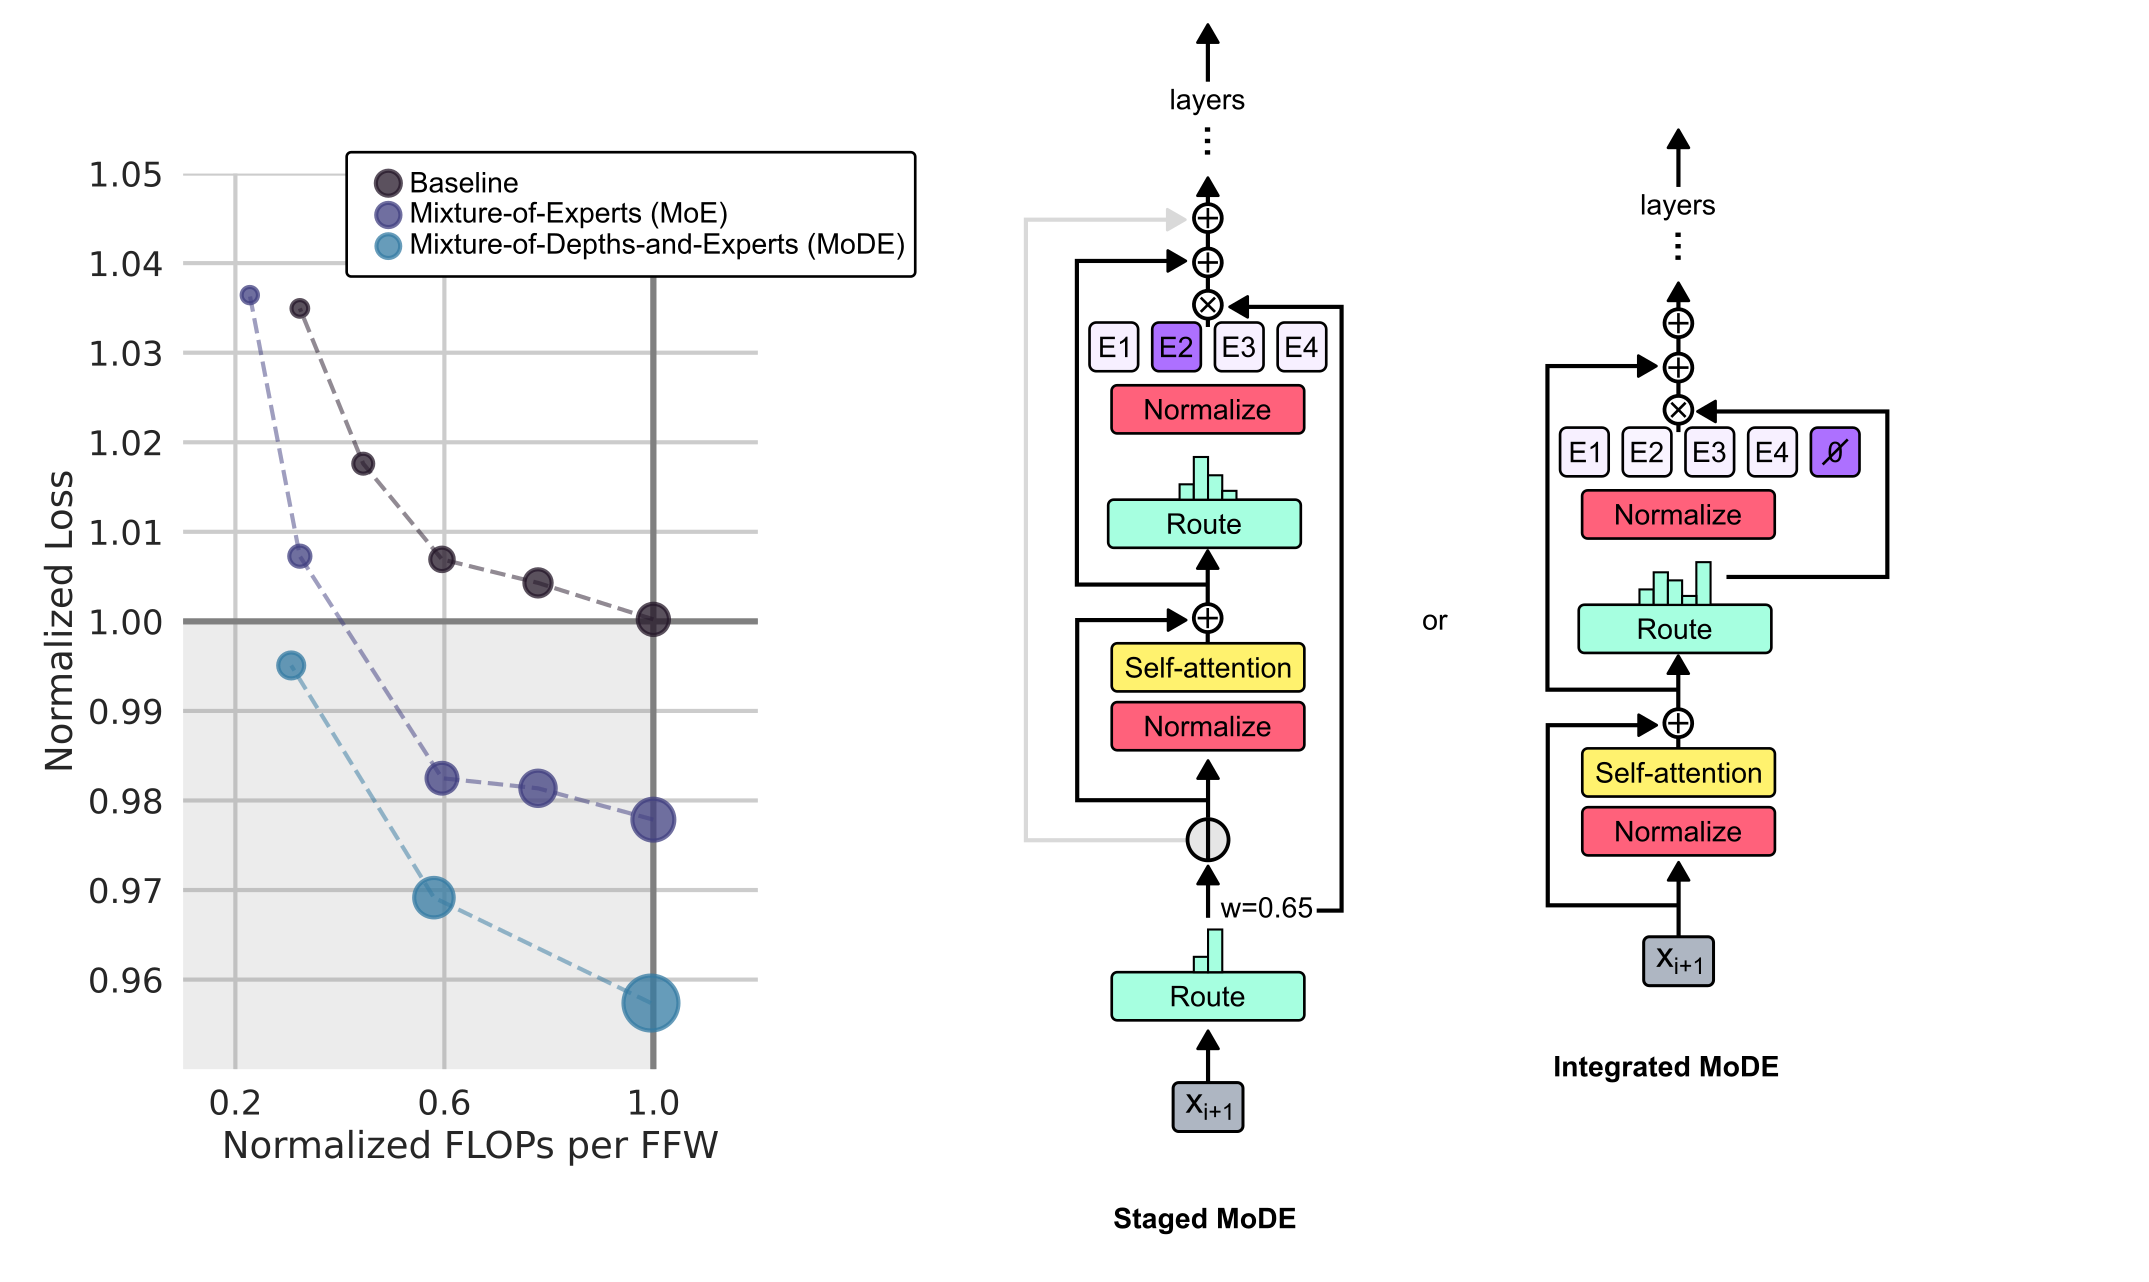
\includegraphics[width=\textwidth]{mode.png}
\caption{\textbf{مزيج الأعماق والخبراء (MoDE).} يمكن تنفيذ تقنية MoD إلى جانب MoE (تشكل معًا نماذج MoDE) بطريقتين بسيطتين: مرحلي، والذي ينفذ أولاً آلية MoD قبل آلية MoE، ومتكامل، والذي يستخدم عملية توجيه واحدة لتوجيه الرموز إما إلى الخبراء أو عمليات عدم التشغيل.}
\label{fig:mode}
\end{figure}
يمكن دمج تقنية MoD بشكل طبيعي مع نماذج MoE (تشكل معًا نماذج MoDE) بالإضافة إلى المحولات العادية. في الشكل \ref{fig:mode} نقدم نتائج توضح أن تحسينات الأداء التي توفرها MoD تتراكم مع تلك الخاصة بـ MoE. جربنا نوعين: في MoDE المرحلي، الذي يوجه الرموز حول أو نحو الكتل قبل خطوة الانتباه الذاتي، و MoDE المتكامل، الذي ينفذ توجيه MoD عن طريق دمج "خبراء عدم التشغيل" بين خبراء MLP التقليديين. الأول مفيد لأنه يسمح للرموز بتخطي خطوة الانتباه الذاتي، بينما الأخير مفيد لأنه يبسط آلية التوجيه. لاحظنا أن تنفيذ MoDE بالطريقة المتكاملة كان أفضل بشكل واضح من مجرد تقليل سعة الخبراء في نماذج MoE التقليدية، والاعتماد على إسقاط الرموز لتنفيذ التوجيه المتبقي. نعتقد أن هذا بسبب أنه مع آلية MoDE المتكاملة، تتعلم الرموز بشكل صريح اختيار المسار المتبقي حول الخبراء، بدلاً من تفضيل خبير ولكن يتم إسقاطها عند تنفيذها كتخفيض للسعة.

\section{المناقشة}
تظهر محولات مزيج الأعماق تجريبيًا أنه يمكن للمرء تحسين أداء الأساس الأمثل isoFLOP باستخدام نماذج تستخدم عددًا أقل من FLOP لكل تمرير أمامي. هذا يعني أنه --- لميزانية تدريب FLOP معينة --- يمكننا تدريب نماذج تكون أسرع وأفضل أداءً من نظيراتها الأساسية. في السابق، لتدريب نماذج تكون أسرع وبنفس جودة أو أفضل من النماذج المثلى isoFLOP، كان على المرء استخدام حوسبة فائضة لـ \emph{الإفراط في تدريب} النماذج الأصغر (من الجدير بالذكر أن تقنية الإفراط في التدريب هذه لا تزال ممكنة مع محولات MoD، ويجب أن تتراكم مكاسب السرعة).

بينما تتطلب محولات MoD عددًا أقل من FLOP لكل تمرير أمامي، لا يمكن للمرء التخلي عن FLOP بشكل عشوائي. بدلاً من ذلك، من الضروري استخدام آليات التوجيه المتعلمة --- تمامًا كما هو الحال في محولات مزيج الخبراء --- لتحديد ما إذا كان ينبغي للرمز المشاركة في الانتباه الذاتي و MLP اللاحق (مما يتطلب FLOP)، أم لا (مما يوفر FLOP). يمكننا بعد ذلك استخدام أي FLOP تم توفيرها عن طريق، على سبيل المثال، جعل النموذج أكبر أو تدريبه لفترة أطول. تظهر نتائجنا أن FLOP قد تُستخدم بشكل غير فعال في نماذج المحول العادية، وأنه قد تكون هناك طرق أكثر كفاءة لإنفاقها.

آليات التوجيه المتعلمة هي أحيانًا \textit{غير سببية}؛ أي أن المعلومات حول المستقبل تُستخدم لتحديد قرار توجيه رمز معين. هذا صحيح بشكل عام لآليات التوجيه أعلى $k$، والتي تكون مفيدة لأنها تتجاوز الحاجة إلى خسائر موازنة مساعدة. ومع ذلك، تطرح آليات التوجيه أعلى $k$ صعوبات في أخذ العينات التراجعي بعد التدريب، حيث يستحيل استخدام معلومات حول هويات الرموز المستقبلية لتحديد قرارات التوجيه. في هذا العمل، نظهر أنه يمكن للمرء استخدام مخطط توجيه أعلى $k$ بنجاح أثناء التدريب، ولكن لا يتطلب ذلك أثناء أخذ العينات التراجعي لاحقًا. إما أن مصنف مساعد بسيط، أو خسارة مساعدة على الموجه، يكفي لتعلم قرارات التوجيه أعلى $k$ بحيث يمكنه تقليد قرارات أعلى $k$ أثناء أخذ العينات التراجعي، مع تدهور أداء ضئيل إلى معدوم.

بشكل حدسي، قد يتعلم الرمز التوجيه حول الكتل لأن التنبؤ الذي يتم إجراؤه في تلك الخطوة أسهل، وبالتالي، لا يتطلب الكثير من الحوسبة. ومع ذلك، هذه الإستراتيجية ليست بالتأكيد كل ما تتعلمه الشبكة. إذا لم يشارك الرمز في الانتباه الذاتي عند كتلة معينة، فلن تتمكن الرموز اللاحقة أيضًا من الانتباه إليه. وبالتالي، فإن ما إذا كانت الرموز تقرر التوجيه أم لا يؤثر على كل من تنبؤ الخطوة الحالية والتنبؤات المستقبلية عبر الانتباه الذاتي السببي، وكيف توازن الشبكة بين هذه التأثيرات يسترشد بتأثيرها على هدف نمذجة اللغة الشامل.

يفتح هذا الاستبصار الباب أمام نسخ MoD التي تفصل التوجيه للاستعلامات والمفاتيح والقيم. على سبيل المثال، ربما يفضل الرمز أن يكون من بين الاستعلامات، ولكن ليس المفاتيح، لحساب انتباه ذاتي معين. يمكن للمرء أن يتخيل توسيع هذه الفكرة أكثر في مجال "الذاكرة طويلة المدى": ربما تكون هناك رموز ستكون قيمة للغاية كمفاتيح، بغض النظر عما إذا كان من المفيد أن تكون أيضًا من بين الاستعلامات في خطوة حدوثها. يمكن أن يكون التوجيه المتعلم آلية قوية لتحديد ما قد تكون عليه هذه الرموز، وربما توجيهها إلى ذاكرة تخزين طويلة الأجل تكون متاحة أثناء الانتباه الذاتي في المستقبل. إحدى مزايا مثل هذا النهج للذاكرة طويلة المدى هي أن الرموز تقرر مرة واحدة، في لحظة "ترميز الذاكرة"، ما إذا كان ينبغي استرجاعها في المستقبل. هذا أكثر كفاءة من الناحية الحسابية من إجراء بحث كامل على أساس المحتوى عبر ذاكرة تخزين مؤقت كاملة لكل خطوة في المستقبل، ويمكن أن يكون خطوة نحو زيادة طول السياق المتاح لتقديم التنبؤ بشكل كبير.

على عكس محولات MoE التي توجه بين نفس الحساب الفعال (عادة MLPs)، تظهر محولات MoD قيمة التوجيه بين أنواع مختلفة من الحسابات. في هذا العمل كانت الأنواع إما كتلة محول تقليدية، أو حساب عدمي (يعادل وظيفيًا الضرب في الصفر). ومع ذلك، يمكن للمرء أن يتخيل توسيع هذه الفكرة أكثر عن طريق التوجيه بين المزيد من أنواع الحساب. على سبيل المثال، ربما يتم توجيه بعض الرموز إلى وظائف "بحث الذاكرة"، ويتم توجيه البعض الآخر إلى وظائف "استخدام الأداة". بشكل عام، توفر آلية التوجيه التي نشرناها مقبضًا لضبط أنواع الحسابات المتاحة للشبكة وتكلفتها النسبية (في إجمالي FLOP)؛ إذا أراد المرء إدخال حساب مكلف، فيمكن تعويض ذلك عن طريق تعيين سعته إلى مقدار صغير، وبالتالي، عن طريق توجيه عدد صغير فقط من الرموز إليه.

بشكل عام، تعد محولات MoD أداة أخرى يمكن استخدامها لضبط حساب النموذج لكل تمرير أمامي (وبالتالي وقت الاستدلال). الآليات المستخدمة لتنفيذ MoD عامة أيضًا، وتفتح الأبواب أمام العديد من الإضافات والتكامل مع التقنيات الأخرى، مثل MoE.
\bibliography{main}

\end{document}
